 
\section*{Aufgabe 1: \emph{Polynom}}

\begin{figure}
\centering
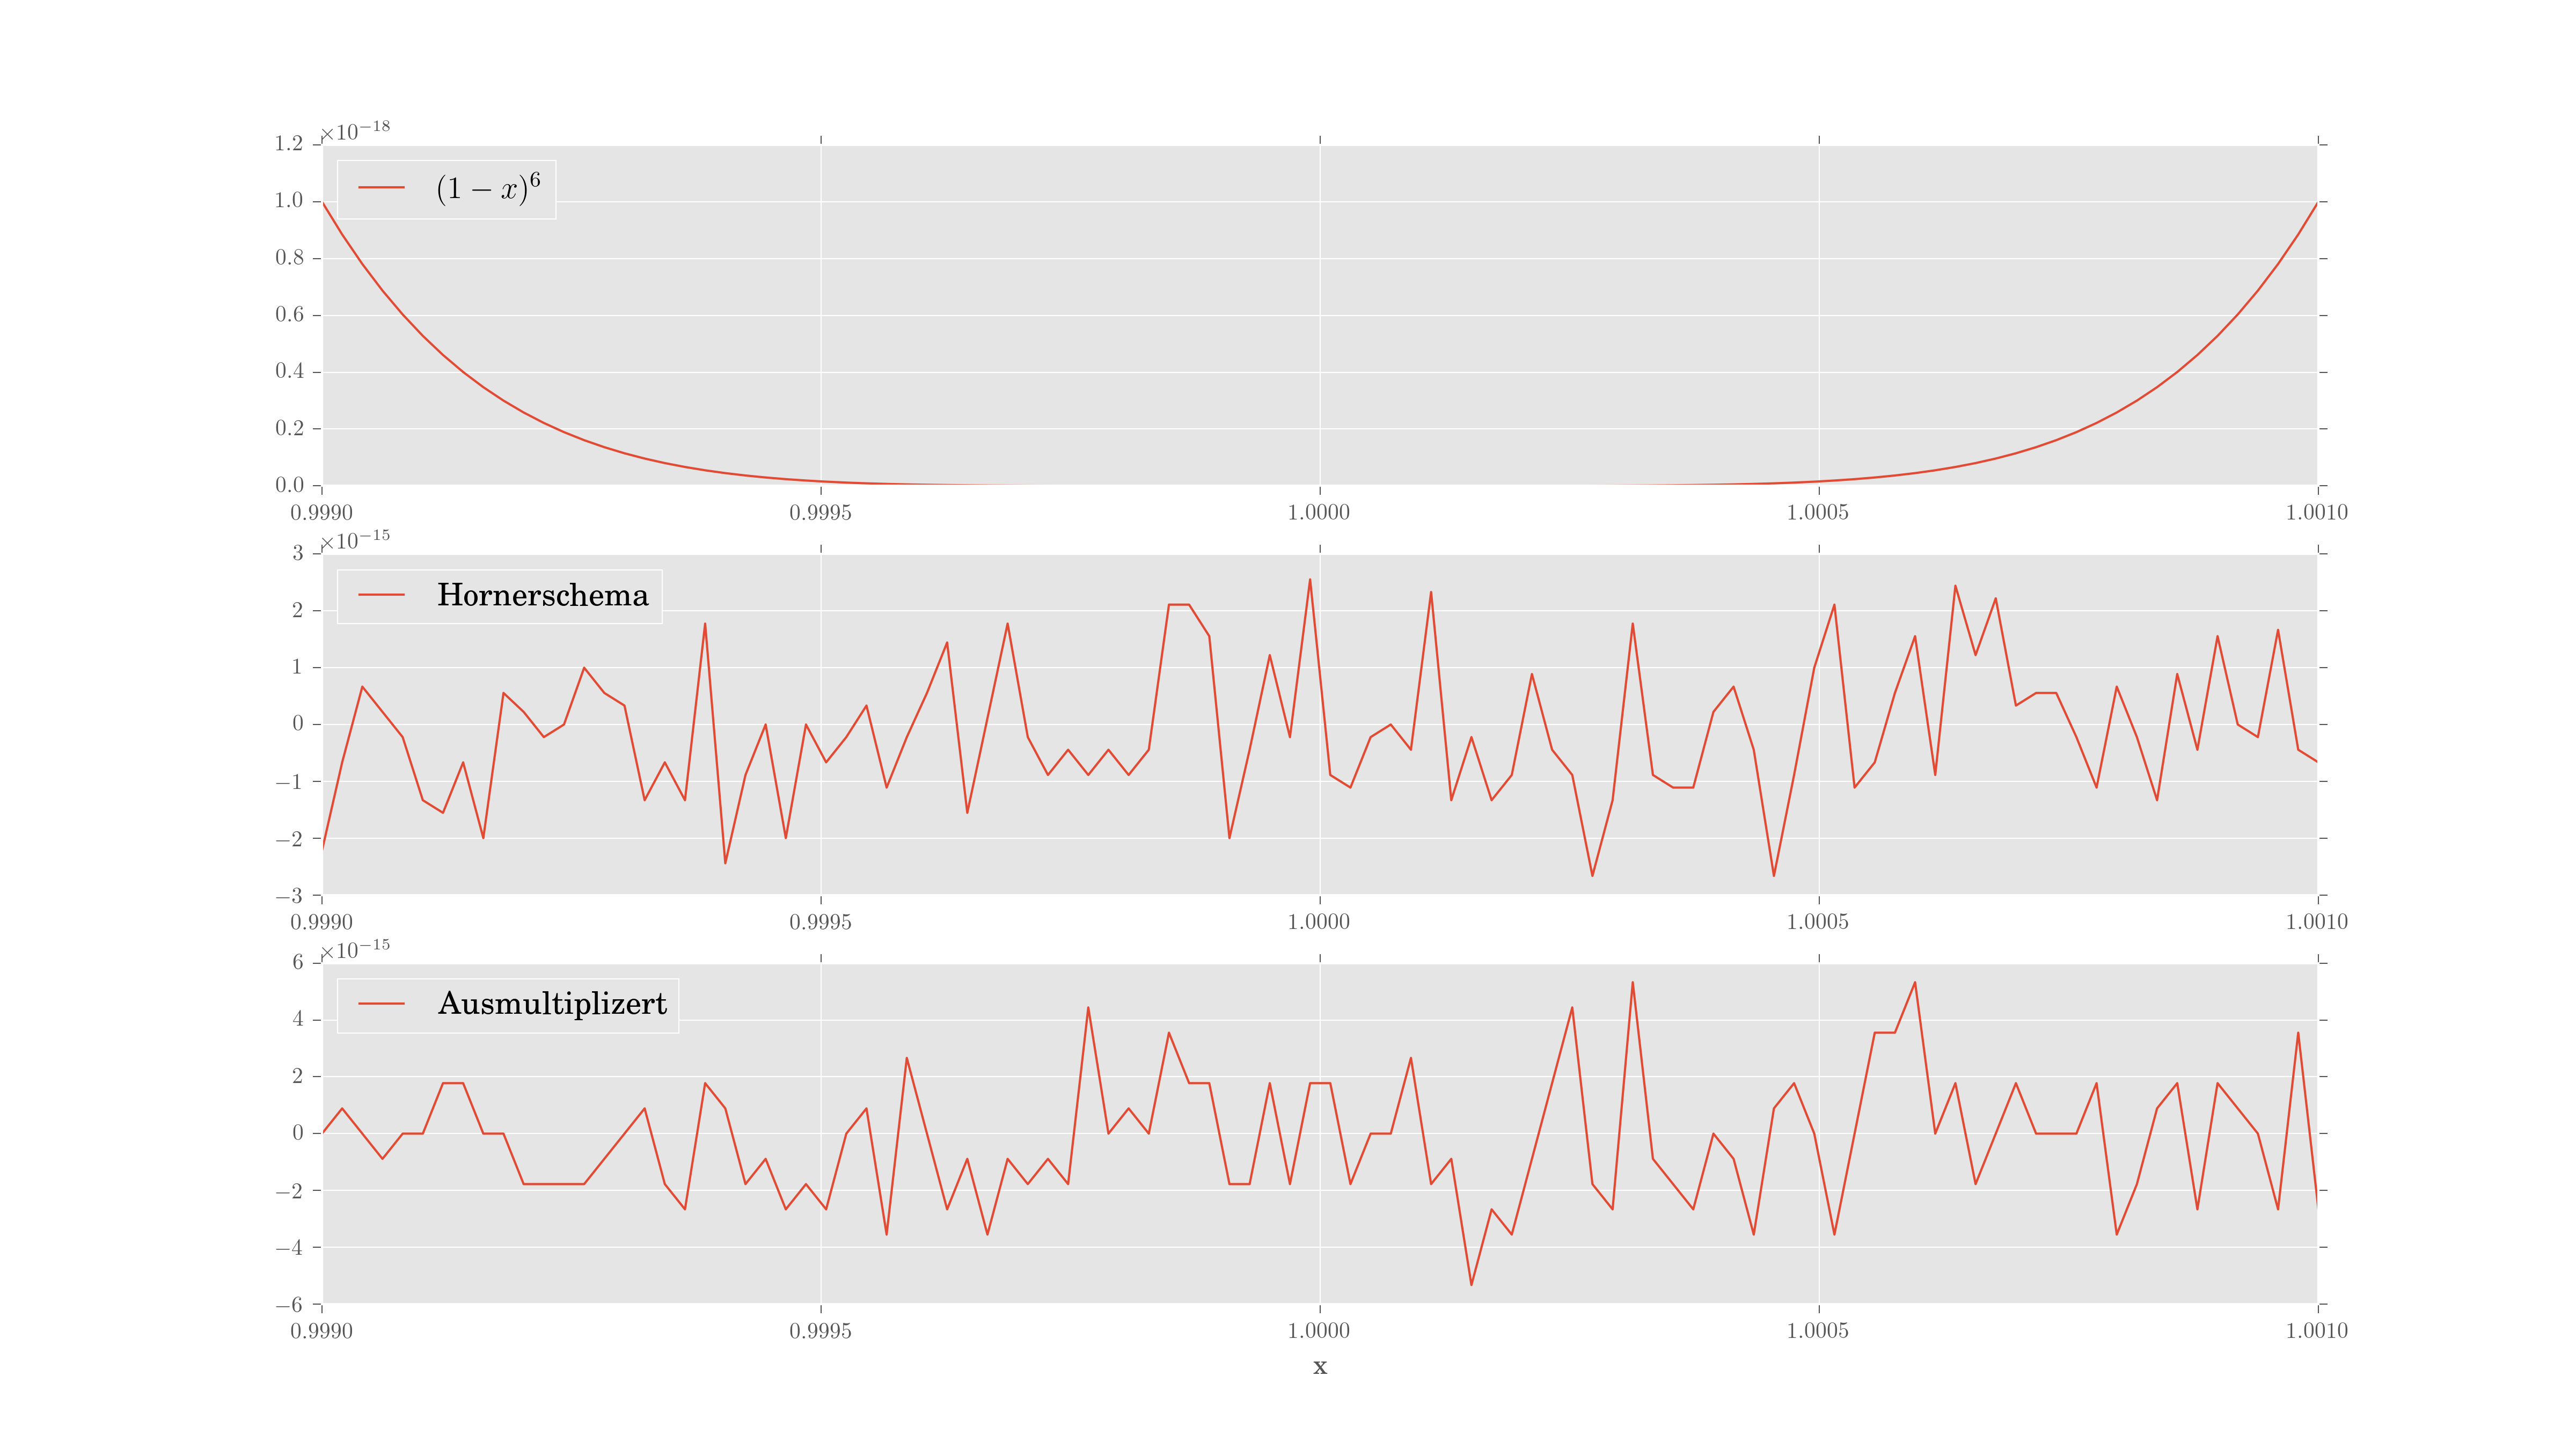
\includegraphics[width=\textwidth]{plot1.png}
\caption{Auswertung des Polynoms $f(x)=(1-x)⁶$. Es wird direkt, durch ausmultiplizieren auf naive Weise und mit dem Horner-Schema berechnet.}
\end{figure}

\section*{Aufgabe 2: \emph{Grenzwert}}

\begin{itemize}
\item[a)] Der Grenzwert der gegebenen Funktion $f(x) = (\sqrt{9-x}-3)\cdot\frac{1}{x} $ berechnet sich mit der Regel von l'Hospital zu 


\begin{equation*}
\lim_{x\to0} (\sqrt{9-x}-3)\cdot\frac{1}{x} = \lim_{x\to0} -\frac{1}{2}\frac{1}{\sqrt{9-x}} = -\frac{1}{6}.
\end{equation*}

\item[b)] \begin{figure}
\centering
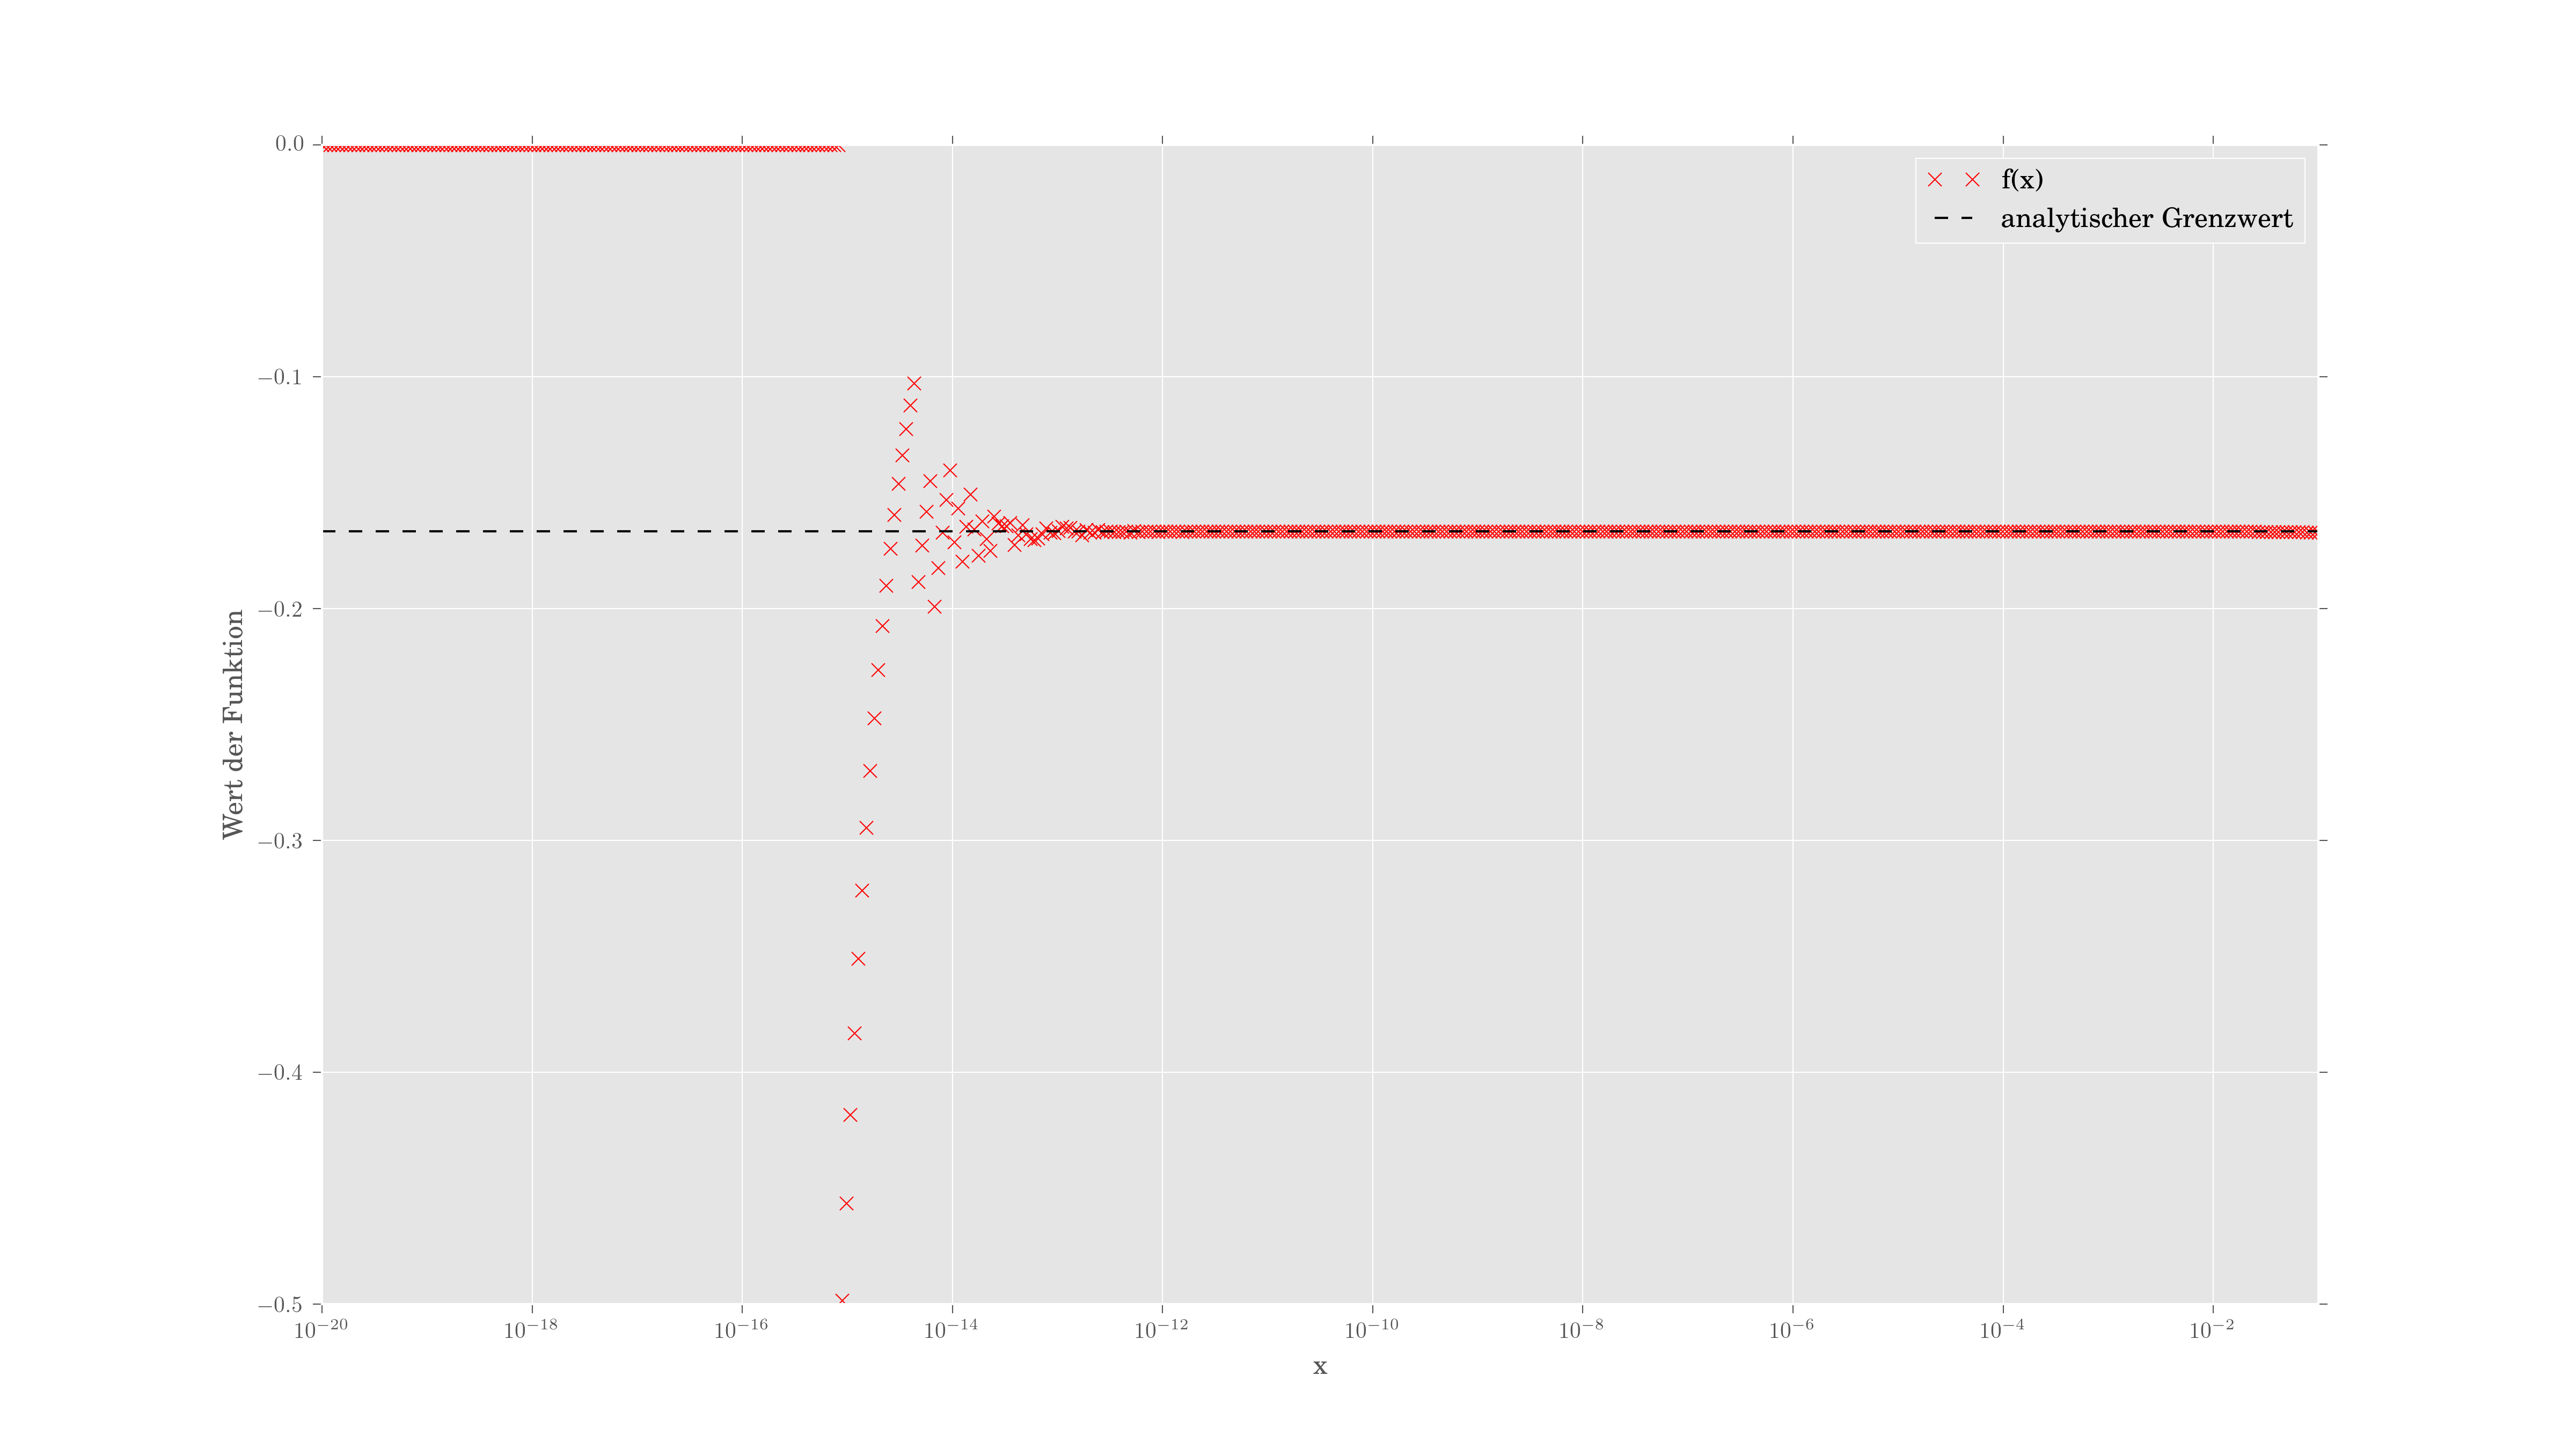
\includegraphics[width=\textwidth]{plot2.png}
\caption{Numerische Berechnug des Grenzwertes der gegebenen Funktion. Dazu wurden Werte von $0.1$ bis $10^{-20}$ eingesetzt und das Ergebnis grafisch dargestellt.}
\end{figure}
Die numerische Bestimmung des Grenzwertes scheitert für Werte von $x<10^{-13}$, da durch sehr kleine Zahlen dividiert wird.
\end{itemize}

\section*{Aufgabe 3: \emph{Numerische Instabilität}}

Die Funktionen liefern für unterschiedliche Bereiche numerische Ergebnisse, die um nicht mehr als $1\%$ vom algebraischen Werte abweichen bzw. für die $f(x)=0$ oder $g(x)=0$ gilt.

\begin{itemize}

\item[a)] Für die Werte $10^{-20}\leq x \leq 1000$ weicht $f(x)$ nur um $1\%$ vom algebraischen Wert ab.\newline\newline
Für die Werte $1000000\leq x \leq 10^{20}$ gilt $f(x)=0$.

\item[b)] Für die Werte $0.0001\leq x \leq 10^{20}$ weicht $g(x)$ nur um $1\%$ vom algebraischen Wert ab.\newline\newline
Für die Werte $10^{-20} \leq x \leq 10^{-6}$ gilt $g(x)=0$.

\end{itemize}

\begin{figure}
\centering
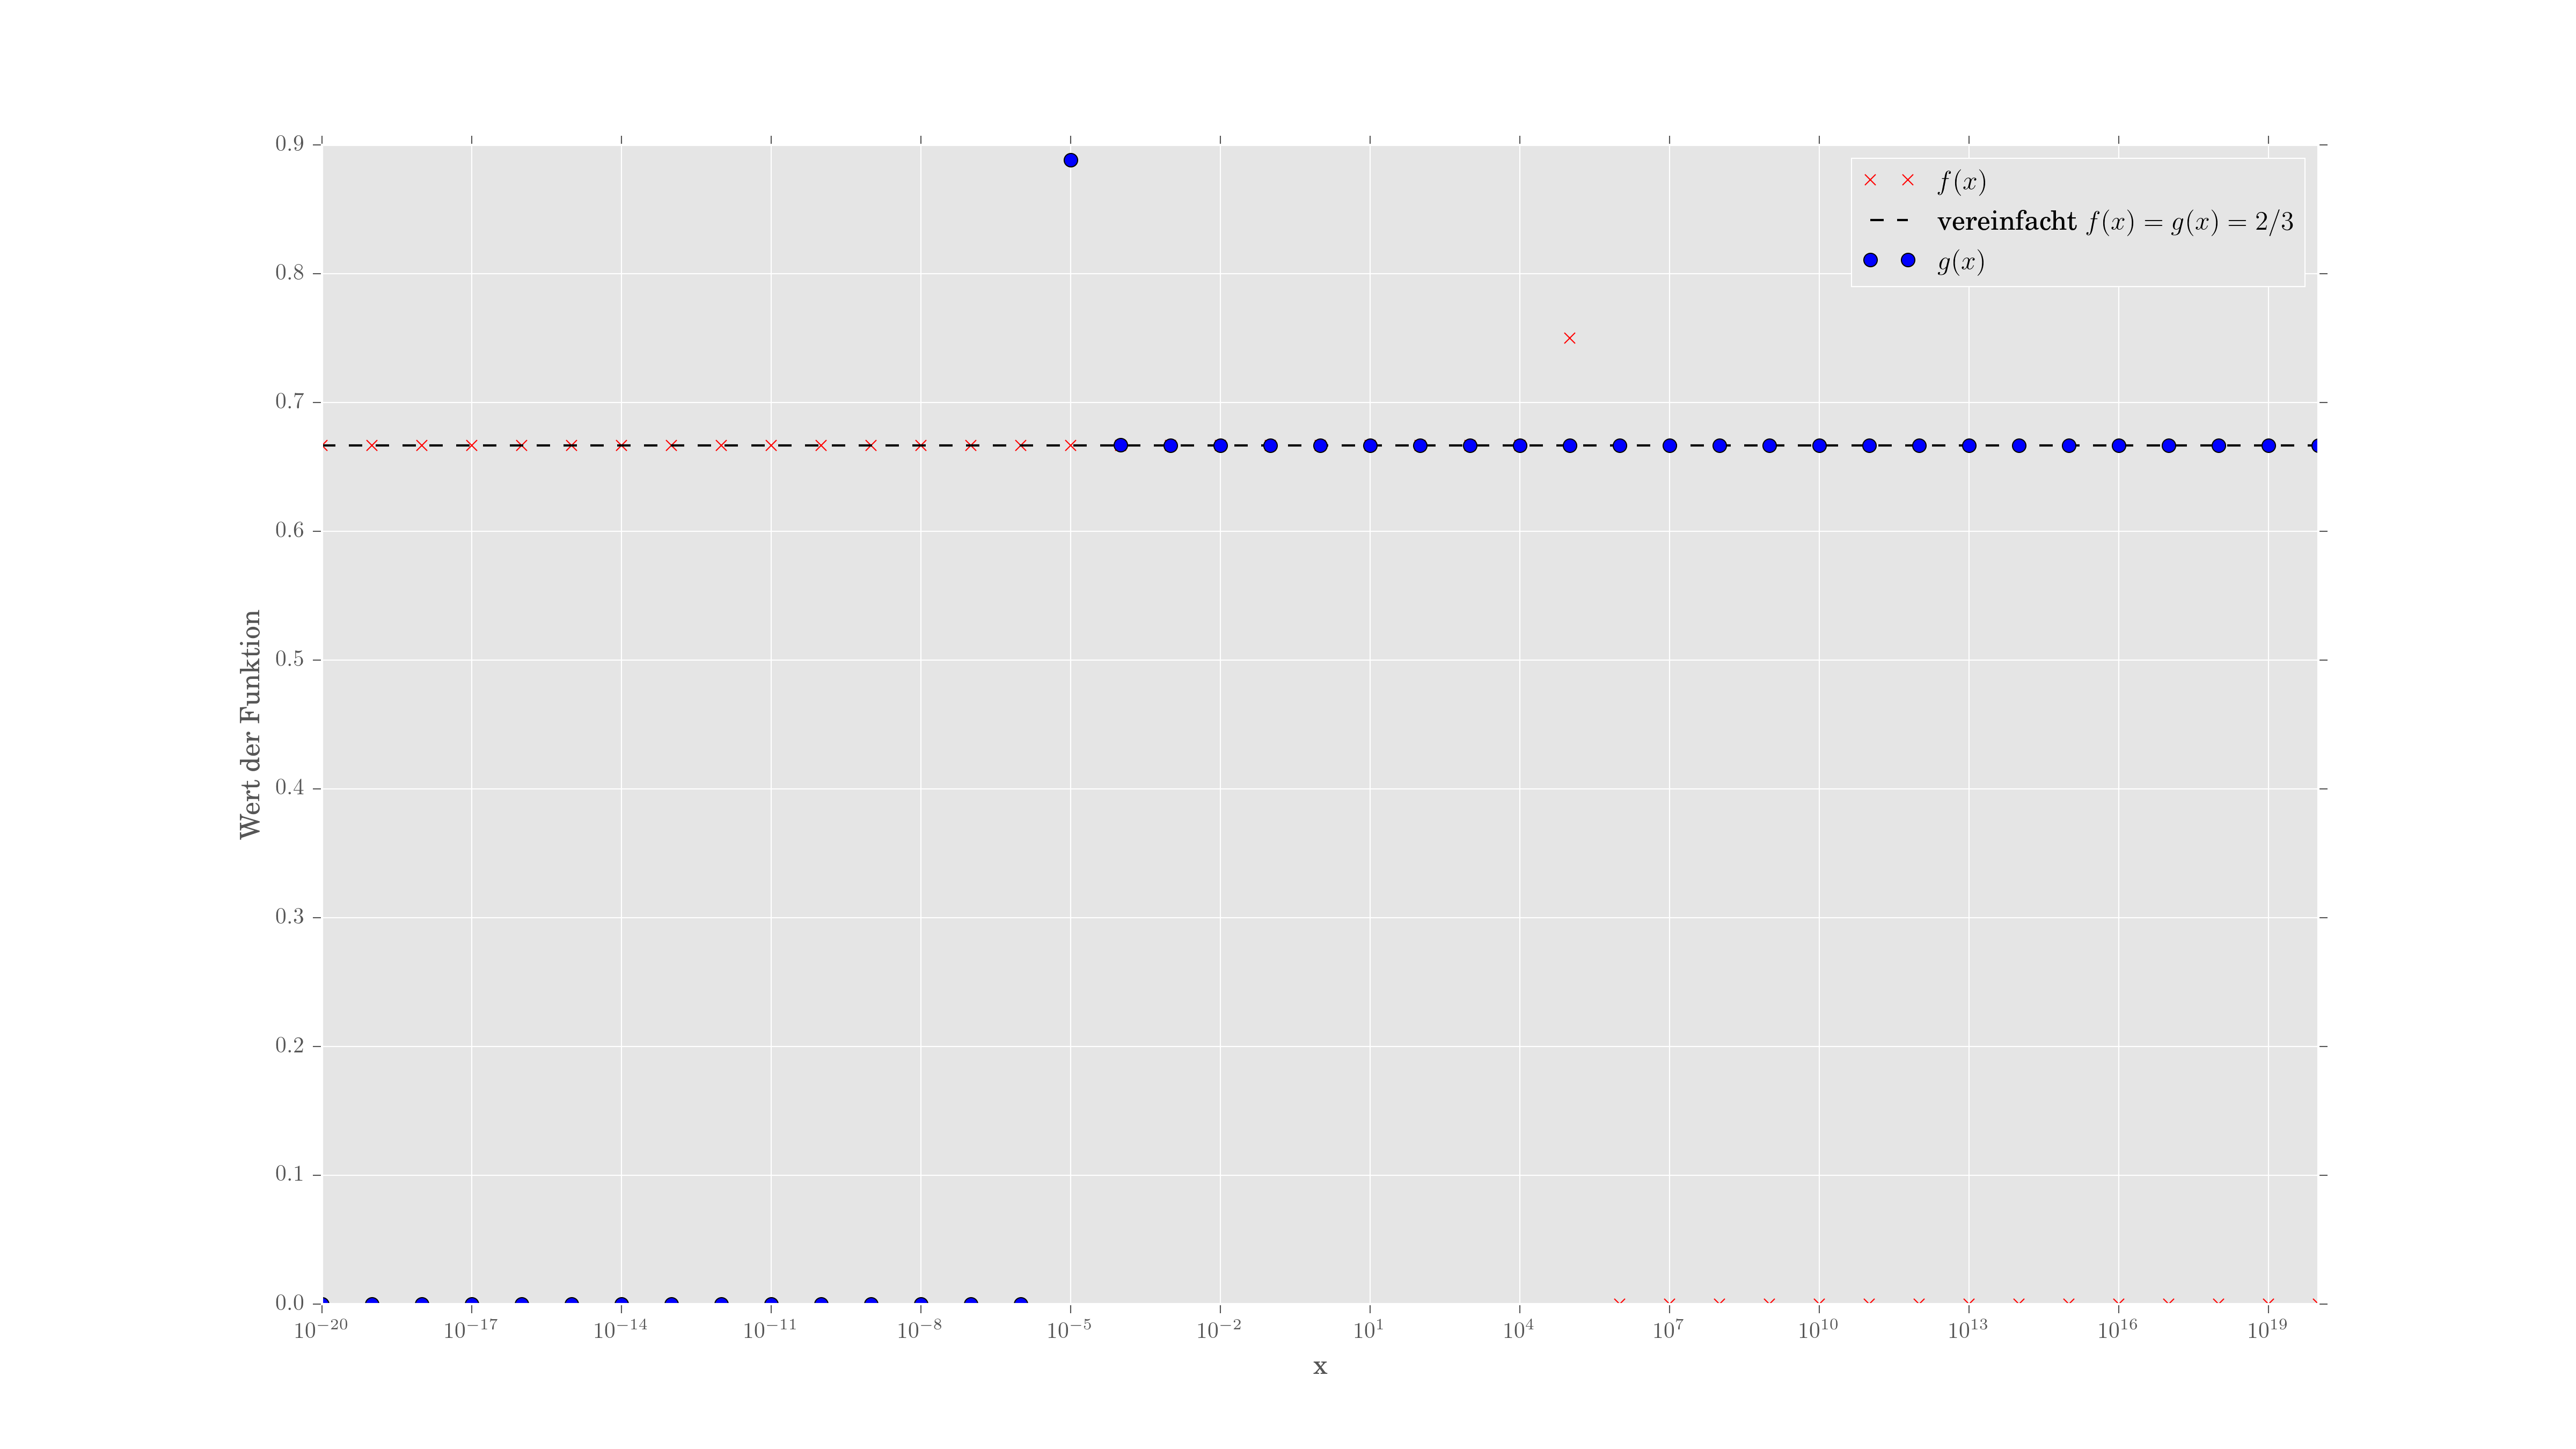
\includegraphics[width=\textwidth]{plot3.png}
\caption{Auswertung der Funktionen $g(x)$ und $f(x)$ im Vergleich mit dem analytischen Wert.}
\end{figure}


\section*{Aufgabe 4}

\begin{itemize}

\item[a)] Die Gleichung 
\begin{equation*}
\frac{\mathup{d}\sigma}{\mathup{d}\Omega}=\frac{\alpha²}{s}\left(\frac{2+\sin²{\theta}}{1-\beta²\cos²{\theta}}\right)
\end{equation*}

ist numerisch instabil für $\beta²\cos²{(\theta)}\approx 1$, d.h. für sehr kleine Werte im Nenner. 
Für $E_e=\SI{50}{\giga\electronvolt}$ ist die Gleichung bei $\theta=0$ und $\theta=n\pi$ mit $n\in{R^+}$ numerisch instabil.

\item[b)] 
\begin{align*}
\frac{\mathup{d}\sigma}{\mathup{d}\Omega}=&\frac{\alpha²}{s}\left(\frac{2+\sin²{\theta}}{1-\beta²\cos²{\theta}}\right)
=\frac{\alpha²}{s}\left(\frac{2+\sin²{\theta}}{(\sin²{\theta}+\cos²{\theta}-\beta²\cos²{\theta}}\right)\\
=&\frac{\alpha²}{s}\left(\frac{2+\sin²{\theta}}{\cos²{\theta}(\sin²{\theta}+1-\beta²)}\right)
=\frac{\alpha²}{s}\left(\frac{2+\sin²{\theta}}{\cos²{\theta}(\sin²{\theta}+\gamma^{-2})}\right)\\
=&\frac{\mathup{d}\sigma}{\mathup{d}\Omega}_{neu}
\end{align*}
\newpage
\item[c)] Siehe Abbildung \ref{1} und \ref{2}.

\item[d)] Berechnung der Konditionszahl über
\begin{equation*}
K=\abs*{x\frac{f'(x)}{f(x)}},
\end{equation*}
wobei die Gleichung $\frac{\mathup{d}\sigma}{\mathup{d}\Omega}_{neu}$ benutzt wird.
\begin{equation*}
K=\abs*{\theta\frac{\left(- 4 \gamma^{2} + 6\right) \sin{\left (\theta \right )} \cos{\left (\theta \right )}}{\left(\gamma^{2} \sin^{2}{\left (\theta\right )} + \cos^{2}{\left (\theta \right )}\right) \left(\sin^{2}{\left (\theta \right )} + 2\right)})}
\end{equation*}

\item[e)] Siehe Abbildung \ref{3} und \ref{4}. Für $\Theta\leq \pi$ ist $K\ll 1$, d.h. in diesem Bereich werden Fehler gedämpft. Bei $\Theta= \pi$ steigt $K$ auf Werte $K\geq1$. Hier werden die Fehler verstärkt; das Problem ist schlecht konditioniert.
\end{itemize}

\begin{figure}
\centering
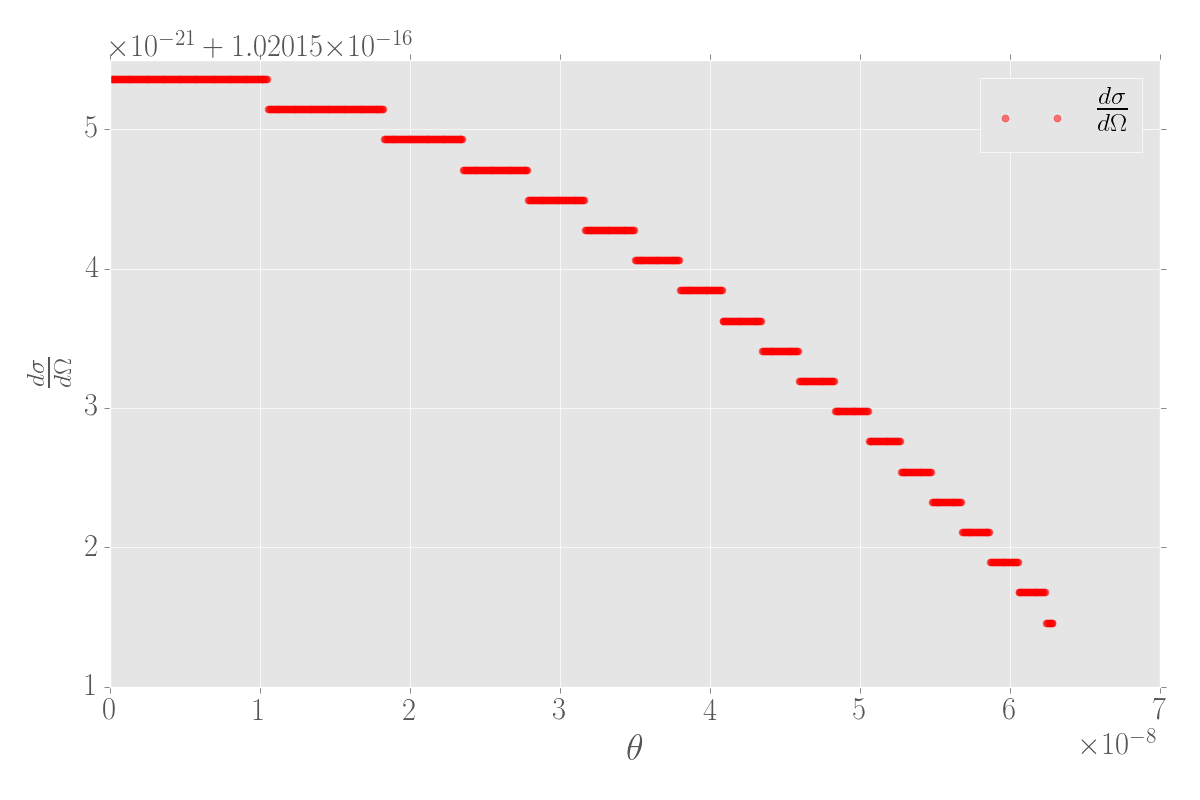
\includegraphics[width=0.8\textwidth]{plot4_c1.png}
\caption{Darstellung von $\frac{\mathup{d}\sigma}{\mathup{d}\Omega}$ für $0\leq\Theta\leq n\pi$.}
\label{1}
\end{figure}

\begin{figure}
\centering
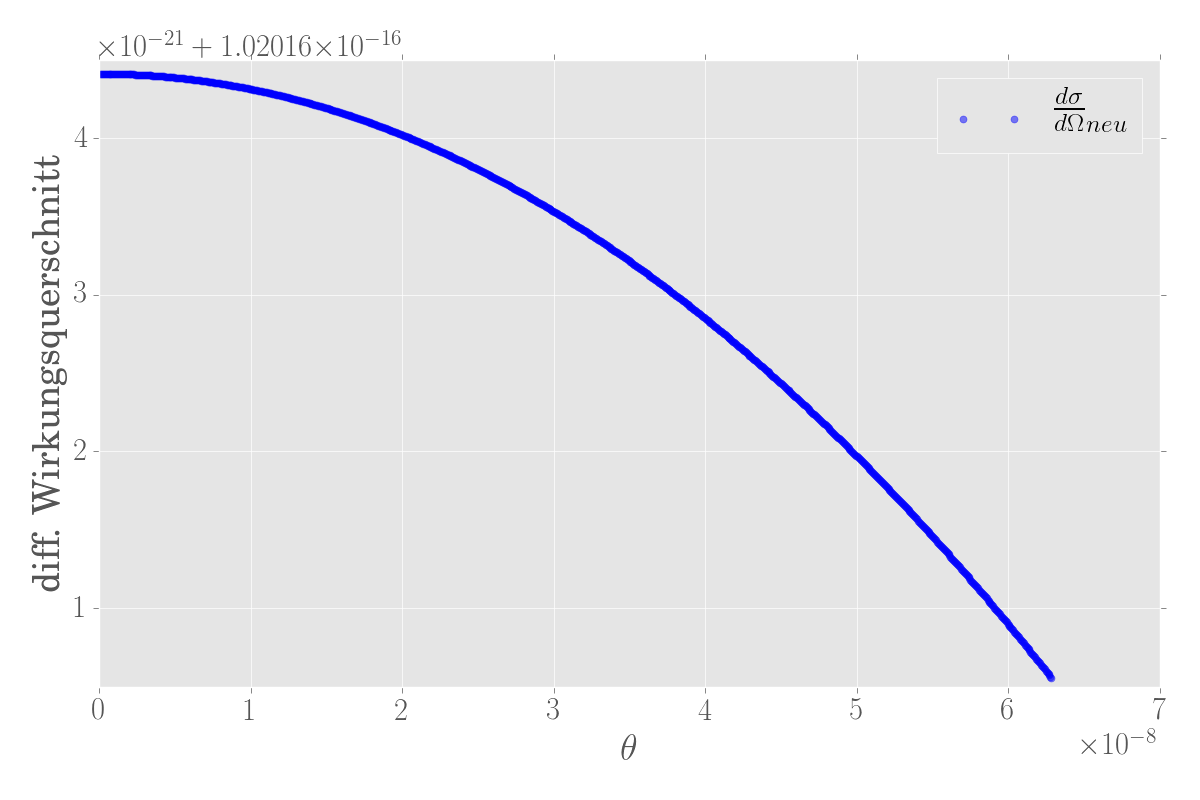
\includegraphics[width=0.8\textwidth]{plot4_c2.png}
\caption{Darstellung von $\frac{\mathup{d}\sigma}{\mathup{d}\Omega}_{neu}$ für $0\leq\Theta\leq n\pi$.}
\label{2}
\end{figure}

\begin{figure}
\centering
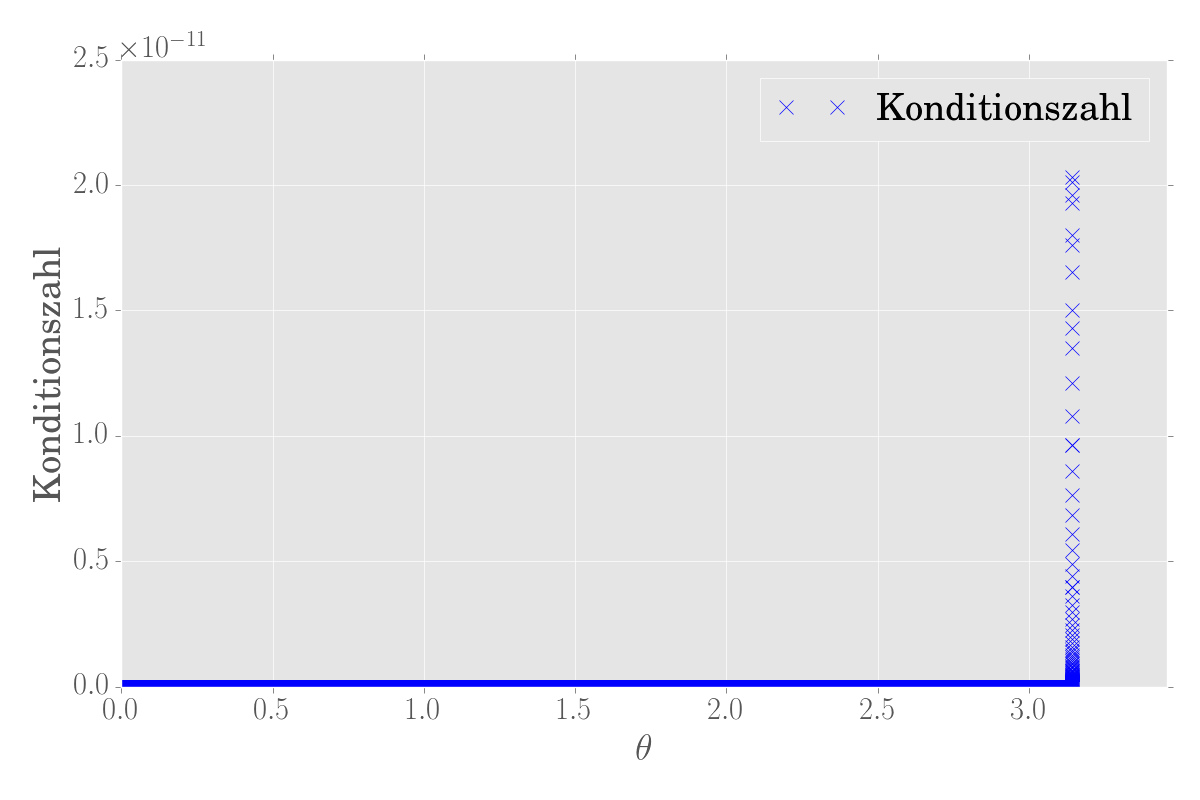
\includegraphics[width=0.8\textwidth]{plot4_e.png}
\caption{Darstellung der Konditionszahl von  $\frac{\mathup{d}\sigma}{\mathup{d}\Omega}_{neu}$.}
\label{3}
\end{figure}

\begin{figure}
\centering
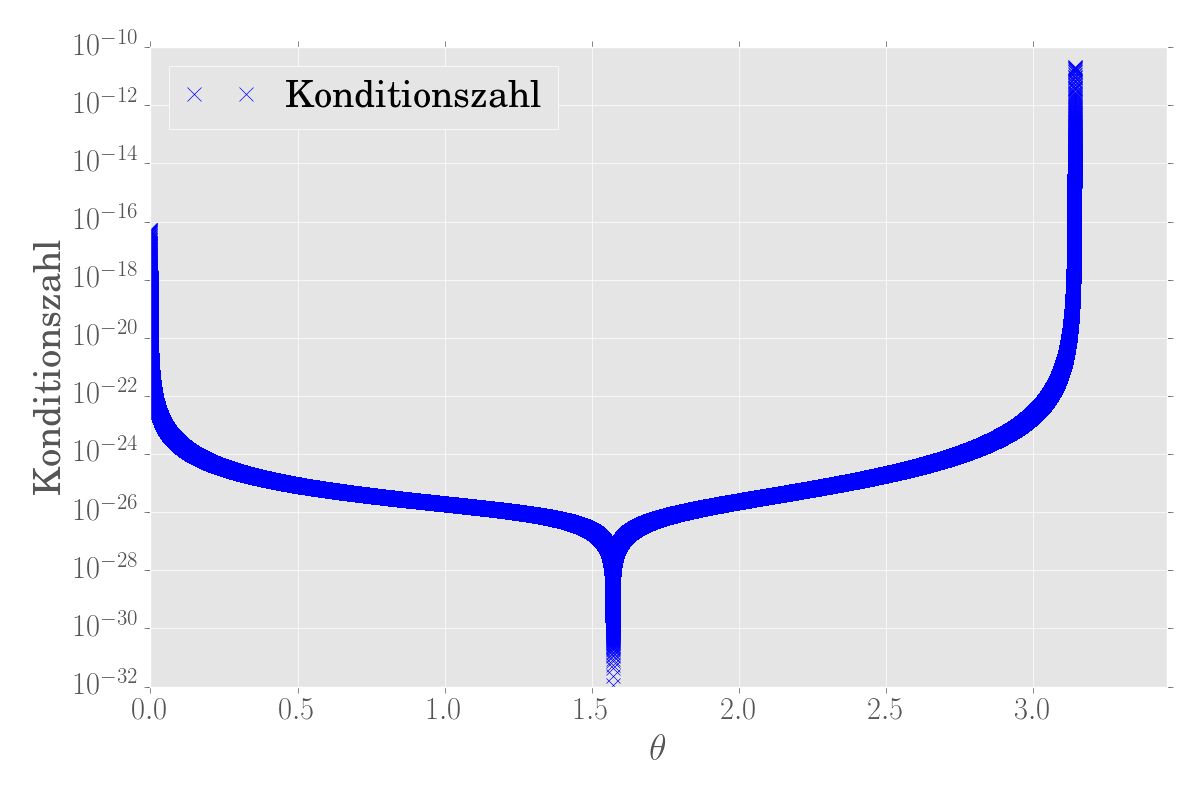
\includegraphics[width=0.8\textwidth]{plot4_elog.png}
\caption{Darstellung der Konditionszahl von  $\frac{\mathup{d}\sigma}{\mathup{d}\Omega}_{neu}$ mit logarithmischer $y$-Achse.}
\label{4}
\end{figure}